\documentclass[a4paper]{article}
% Use utf-8 encoding for foreign characters
\usepackage[utf8]{inputenc}

% Setup for fullpage use
\usepackage{fullpage}

\usepackage{color}
\usepackage{index} % use index package to create indices
\newindex{todo}{tod}{tnd}{TODO List} % start todo list
\newindex{fixme}{fix}{fnd}{FIXME List} % start fixme list
\newcommand{\todo}[1]{\textcolor{blue}{TODO: #1}\index[todo]{#1}} % macro for todo entries
\newcommand{\fixme}[1]{\textcolor{red}{FIXME: #1}\index[fixme]{#1}} % macro for fixme entries
\usepackage{amsfonts}
\usepackage{pifont}
\usepackage{boxedminipage}
% If you want to generate a toc for each chapter (use with book)
\usepackage{minitoc}
% Package for including code in the document
\usepackage{listings}

\title{Automated Theorem Prover For Euler Diagrams}
\author{Sasan Padidar}
\usepackage{graphicx}

\begin{document}
\maketitle
\tableofcontents

\section{Introduction} % (fold)
\label{sec:introduction}

\subsection{General}

Software reliability arguably is one of the most important issues in software engineering. The idea of producing 100\% reliable software has been in computer science for a long time. According to ANSI, Software Reliability is defined as: the probability of failure-free software operation for a specified period of time in a specified environment \cite{ANSI_91}. Although Software Reliability is defined as a probabilistic function, and comes with the notion of time, it must be noted that, it  differs from traditional “Hardware Reliability”, “Software Reliability” is not a direct function of time. Electronic and mechanical parts may become "old" and wear out with time and usage, but software will not wear-out during its life cycle. Software will not change over time unless intentionally changed. This makes software reliability a critical point in software production because software in many cases might last for a long period of time. Not being certain about the reliability of software will cause problems during the life cycle of the software and will have significant costs for its maintenance.  Therefore there is a great deal of benefits in producing reliable software both for the user and the designers.

This need for creating reliable software has led many mathematicians, computer scientists and software engineers to create new methods to properly specify and test software. There are a number of different approaches for specifying software in order to eliminate potential errors from the design and creating specific and clear guidelines for creating functions. These methods have proven to be significantly helpful in creating reliable software and they are being used mainly on safety critical systems currently.

\section{Software Specification}

The aim of software specification is to create a create a (high-level) model serving to specify an abstract architecture for the required system where its outcome must be understood \cite{Howse_2005}. 

Producing reliable software in non-safety critical systems must be as important as safety critical systems because these systems are going to exists for a while and they must be in their best working condition. This reduces maintenance cost and also makes users more satisfied. In order to have 100\% reliable software there must be a clear detailed specification for the entire system. There also has to be a set of defined metrics for creating software. The set of metrics must clearly specify the expectation boundary and the absolute purpose of the software. Also there must  exists a system that can ensure the reliability of the software automatically because if the current methods evolve to a more complex method they will discourage engineers to use them as it will make their job even more complex and expensive [Personal Opinion].


\subsection{Formal Languages}

Specification can be written using a number of formal languages which include OCL, ML, etc. A formal language is a set of words i.e. finite strings of letters or symbols \cite{Mateescu_1997}. By using the words and symbols it is possible to represent different operations which can be used for specifying a particular operation.
\linebreak 
Formal languages normally contain the following symbols to represent the idea: $\vee, \wedge, \in, \lambda, \cap, \ni, \subset, \supset$. This is just for demonstrating what symbols are included in symbolic logic, there are many more symbols as well. 

\subsection{Visual Modelling}
 
As stated in the “formal languages” section using formal languages is generally difficult and hard to read. This has led to a number of researchers (mainly mathematicians) to look for an easier method of specifying software which offers the same level of formalism and accuracy as formal languages do. The result of this research is using visual modelling namely diagrammatic modelling rather than symbolic modelling. Researches that are currently being carried out on use of diagrams for  software specification are producing some promising tools that can be used to specify software formally. This method of specification uses diagrams, mainly Euler/Ven diagrams to represent different aspects of  the system that is being specified and then by applying diagrammatic reasoning rules to each diagram the specification can be proved to be correct.
 
This system has a number of advantages which include:
\begin{enumerate}
\item Specification can be understood more easily by looking at a number diagrams rather than reading the symbolic statements that other languages use.
\item Reading and understanding the specification becomes much faster than using symbolic statements.
\item It is significantly easier and faster to produce the specification using diagrams rather than using the symbols.
\end{enumerate}

This makes specification relatively easier and faster which is quite a compelling reason for choosing diagrammatic notation as the specification method as the engineers are after an easier and faster specification method. These advantages are all arguable, they should not be treated as proven facts and they are not the only advantages of the diagrammatic system. Different designers and engineers require different tools in order to produce their specification. It is a scientific fact that different people learn and conceive information in different manners, some people learn visually faster and can remember information visually and this system is just another tool that has to exist for people who are more comfortable with visual information. This diagrammatic system is still being developed and there is a great deal left to be discovered in this area. It is too early to judge whether the diagrammatic system has any particular advantages over symbolic logic and it is difficult to have a compelling scientific fact for designers in symbolic logic to adopt diagrammatic system and use that for their specification work. However it seems that the diagrammatic system and symbolic logic have to coexist to make an efficient specification method. For a more detailed information on diagrammatic system refer to \cite{Aidan_Gem}
   
As explained above in order to use the diagrammatic method it is needed to apply diagrammatic reasoning rules to diagrams to ensure that the specification is correct logically. This means that the designer has to apply rules to each diagram that is supposed to follow from another diagram and prove that the meaning the diagrams imply is correct logically (will be explained in more details). This is currently done manually by the designers which is error prone and is a tedious process. For instance when a designer has specified what should happen after an event in the program has occurred, s/he has to represent the starting state of the program in a diagram and also the desired state after the event has occurred. Then by applying reasoning rules that the diagrammatic system provides s/he can prove whether the diagrams truly follow from one another logically or not. If not that means the specification has errors in it and therefore the program that is written based on that specification has bugs in it.

\subsection{Project Objectives}

This project aims to create an automated  prover for (Euler) diagrams which can prove the correctness of diagrams and can also write the proof. This will make the process of specification much faster and less error prone.The aim of the project is creating a prover for unitary and compound diagrams. 
The advantages that this system has are:

\begin{enumerate}
\item This system will save the designer a lot of time in proving the correctness of the diagrams and allows the designer to spend more time on specification.
\item This system reduces the errors that might occur during the specification process because it can be used to prove the correctness of each step of the design rather than doing it when the specification is done.
\item The designer does not have to know the rules of diagrammatic proof. S/He can just use the prover to see if diagrams follow from each other or not. Comparing to the other formal methods, the designer must be aware of the formal logic behind the language.
\end{enumerate}
Currently there is an automated theorem prover called “Edith” that is a unitary diagram prover written in Java. This project's goal is to create another prover that is for compound diagrams as well as unitary which is open source and has a better structural design compared to Edith. 

\newpage

\section{Visual Modelling}

\subsection{Brief Diagrams History}
After Shin's \cite{Shin_1994} work on demonstrating that it is possible to have a sound and complete diagrammatic logic, diagrams have become a valuable tool to be used in logic. One of the most important reasons that diagrams are used is because of they are much more intuitive to understand compare to symbolic logic. Understanding and using symbolic logic needs the ability to understand and formulate rigorous arguments. As a result of this issue symbolic logic is not accessible to a wide range of users i.e. software engineers, programmers, computer scientists, etc. Software Engineers are used to the idea of using frameworks that are standard in the industry and they can be used to communicate with other software engineers. Having symbolic logic as a framework is just inefficient because of the vast amount of knowledge engineers should have in order to understand  the rigorous arguments and logical statements. Moreover experience has proven that software engineers are more comfortable with visual modelling tools such as the Unified Modelling Language (UML). Considering these facts it seems compelling that there is a need of a diagrammatic system that can represent logical statements. This diagrammatic system has the potential to become the standard modelling framework in the industry and could be beneficial to many potential users due to its rather straight forward, intuitive way of understanding it \cite{Gem_1}.
Figure 1 below demonstrates the difference between understanding the meaning of a diagram compared to a symbolic statement. The diagram below can be interpreted in different ways. An interpretation of it could be “There does not exist any car that is a computer or a PC” in symbolic logic is:
$$ \neg\ni x ((Computer(x) \vee pc(x)) \wedge Car(x))$$
\begin{figure}[h]
\centering
\includegraphics{images/diag2_21.png}
\caption{Not the normal form of the diagram (explained later)}
\end{figure}

\begin{figure}[h]
\centering
\includegraphics{images/diag2_22.png}
\caption{The normal form of the diagram}
\end{figure}

The shaded areas represent emptiness. The normal form and the shading are explained in later.

\subsection{Overview Of Diagrams}
There a number of different diagrams that are used by mathematicians in the area of logic that is related to sets i.e. Ven diagrams, Euler diagrams, Spider diagrams, Johnston diagrams, etcetera. These diagrams all have some advantages and disadvantages in different circumstances. Euler diagrams are the main concern here as this project is about implementing a prover for Euler diagrams. 

\subsection{Euler Diagrams}

The definition of Euler diagrams as described in \cite{Fish_2007} is Euler diagrams are finite collections of simple closed curves (shapes that do not self-intersect) drawn in plane and may also contain shading. Euler diagrams consist of contours and zones. The definitions regarding Euler diagrams are:
\begin{itemize}
\item Contour is a closed curve that represents a set. For instance in the diagram below “A” is a contour.
\item Zone is a finite disjoint sets of contour labels. In other words zones represent different areas in a diagram.
\item Shaded Zone in Euler diagrams means that the specific area in the diagram is empty. In other words the shaded zone means there is no element in that area.
\item Zonal Region is a region that becomes a zone when contours are removed. 
\end{itemize}
For more detail refer to \cite{Fish_2007}

The diagram below is an example of an Euler diagram.

\begin{figure}[h]
\centering
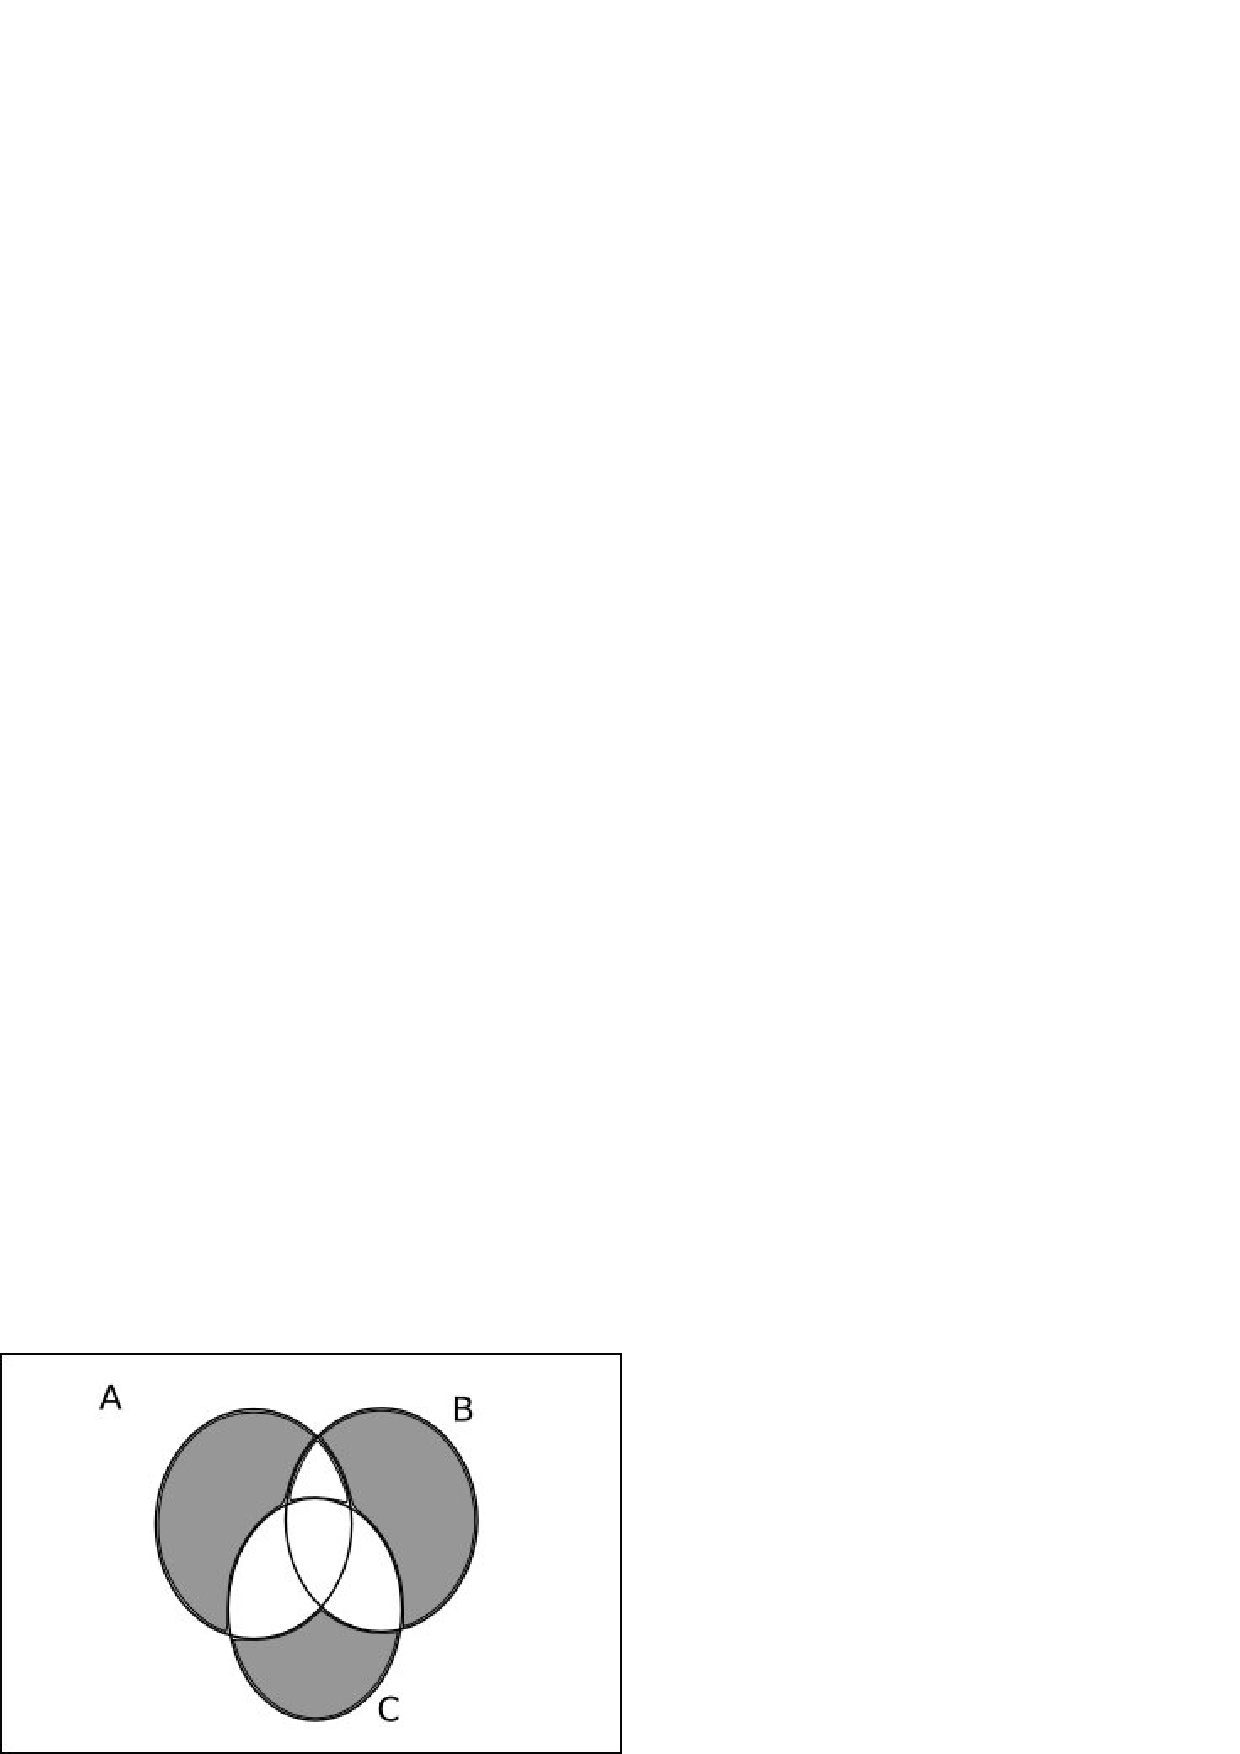
\includegraphics{images/dia2.png}
\caption{An Euler Diagram}
\end{figure}

There might be a slight confusion between Euler diagrams and Venn diagrams because of their similarities. Venn diagrams can be seen as a special case of Euler diagrams, as Venn diagrams must contain all possible zones, whereas Euler diagrams can contain a subset of all possible zones. In Venn diagrams a shaded zone represents an empty set, whereas in an Euler diagram the corresponding zone could be missing from the diagram. This means that as the number of contours increase, Euler diagrams are typically less visually complex than the equivalent Venn diagram, particularly if the number of non-empty intersections is small \cite{Kent_Euler}.

The intersection of the contours in Euler diagrams means that there exists common elements between those particular contours which are basically sets. Each Euler diagram has an abstract syntax which describes the diagram using text rather than pictures. This abstract syntax helps significantly in creation of an automated theorem prover for the diagrams because it provides a structured framework to be used in describing each diagram while trying to prove theorems (this will be explained in the later chapters). To give an example of the abstract syntax, the abstract syntax of the above diagram is written below.
\newline \newline
$contours =  \lbrace A, B, C \rbrace $ \newline
$zones = \lbrace (A , BC) , (B , AC), (C, AB), (AB , C) , (BC , A) , (AC, B), (ABC , ), (  , ABC) \rbrace  $ \newline 
$shaded zones = \lbrace (A , BC), (B , AC) , (C, AB) \rbrace  $ \newline

The abstract syntax of the diagram only puts the diagram in textual format and says nothing else about it. It is still possible to read the abstract syntax as reading the diagram itself. For instance the zone $(A, BC)$ can be read as inside $A$ and outside $B$ and $C$. Zones are put into brackets in the abstract form and the separating comma separates the inside of the zone with its outside. To clarify, the contour label(s) on the right side of the comma are the part of the zone that is being considered but just having that is not enough because the contour(s) might have intersections with other contours that are not being considered. Therefore it is necessary to state on the left side of the comma what contours are not included in the zone.

\subsection{Diagrams}
There are two types of diagrams in this system:
\begin{itemize}
\item Unitary Diagrams: A unitary diagram is just a single (Euler) diagram which is constructed without the use of any operators.
\item Compound Diagrams: A compound diagram is a diagram is a diagram that is constructed using the operators $\wedge or \vee$ or both. The operator $\neg$ can also be used to represent the complement of a diagram.
\end{itemize}

For details about complement operator and understating set theory refer to \cite{Taylor_book}

\subsection{Notations}
The notations that are used in this system are explained below:

\begin{itemize}
\item $ \vee : $ This operator is called the "Or" operator.   \\
\item $ \wedge : $ This operator is called the "And" operator.  \\
\item $ \neg : $ This operator is called the "Not" operator. It is used to represent the complement of its operand (a diagram). \\
\item $ \cup : $ This operator is called the "Union" operator.  \\
\item $ \cap : $ This operator is called the "Intersection" operator. \\
\item $ \leftrightarrow : $ This operator means that the statement is correct in both ways. \\
\end{itemize}

\subsection{Reasoning}

In order to have a formal diagrammatic system it is necessary to have a set of well defined rules that can be used to prove the correctness of diagrams formally. Because of this reasons a number of well defined rules are defined in a number of different papers which include \cite{Fish_2007} and \cite{Gem_Judith}. These rules are significantly helpful in structuring the process of proving (explained in later sections). By substituting different diagrams in different reasoning rules it is possible to prove certain issues about that diagram or diagrams. This depends on the context that the diagrams are being considered. For this project a certain number of rules are used to check if there exists a proof between two or more diagrams. In this project restrictive reasoning rules are used. It is possible to weaken these rules and have a number of different rules called the “relaxed reasoning system” \cite{Fish_2007}.

\subsection{Reasoning Rules}
The rules that are used in the prover are :
\begin{enumerate}
\item Add Contour
\item Remove Contour
\item Add Shaded Zone
\item Remove Shaded Zone
\item Identity Law
\item Complement Laws
\item De Morgan's Laws
\item Involution
\item Distributivity
\item Idempotency 
\item Inconsistency
\item Connecting a diagram
\item Removing a diagram
\end{enumerate}

%%Before explaining the rules it is necessary to know what the symbols used in the rules mean. Explaining the symbols in symbolic logic and then mapping them to their correspondent in diagrammatic logic would be easier to undestand.\\
%%$ \cup : $ in symbolic logic means the unioun of sets. In diagrammatic logic is 
Each rule is explained with examples below in detail:

\subsubsection{Add Contour}
This rule simply adds a new contour to the diagram. Provided that the contour is not already in the diagram.Adding the contour causes each zone to be split into two zones (one inside and one outside the new contour), and shading is preserved \cite{Fish_2007}.
The figures below demonstrates how a new contour is added.
As it is clearly visible the new contour C is added to the diagram and has split all zones into two zones. The abstract syntax of figure \ref{fig:add1} before adding is:\newline
$contours =  \lbrace A, B \rbrace $ \newline
$zones = \lbrace (A , B) , (B , A), (AB , ) , ( , AB) \rbrace  $ \newline 
$shaded zones = \lbrace (AB , ) \rbrace  $ \newline

\begin{figure}[h]
\begin{minipage}[h]{0.5\linewidth}
\centering
\includegraphics[scale=0.5]{images/diag3add1.png}
\caption{Before applying Add contour}
\label{fig:add1}
\end{minipage}
\hspace{0.5cm}
\begin{minipage}[h]{0.5\linewidth}
\centering
\includegraphics[scale=0.5]{images/diag3add2.png}
\caption{After applying Add contour}
\label{fig:add2}
\end{minipage}
\end{figure}

After adding the new contour the abstract syntax becomes:\newline
$contours =  \lbrace A, B, C \rbrace $ \newline
$zones = \lbrace (A , BC) , (B , AC), (C, AB), (AB , C) , (BC , A) , (AC, B), (ABC , ), (  , ABC) \rbrace  $ \newline 
$shaded zones = \lbrace (AB , C), (ABC , ) \rbrace  $ \newline

\subsubsection{Remove Contour}
Removing a contour is the reverse process of adding a contour. All the zones that are involved with that contour will combine with other zones to form a single zone. For all pairs zones that have to combine in order to form a single zone which are both either shaded or nonshaded, the shading is preserved and no new shading is added.\cite{Fish_2007}. In the abstract syntax all the zones that are created by the add contour rule must be removed and all the zones that have the contour label that is being removed in them must be updated to exclude the contour label.

The diagrams below demonstrate removing of contour C. The abstract syntax of figure \ref{fig:add3} before removing the contour is:\newline
$contours =  \lbrace A, B, C \rbrace $ \newline
$zones = \lbrace (A , BC) , (B , AC), (C, AB), (AB , C) , (BC , A) , (AC, B), (ABC , ), (  , ABC) \rbrace  $ \newline 
$shaded zones = \lbrace (AB , C), (ABC , ) \rbrace  $ \newline

\begin{figure}[h]
\begin{minipage}[h]{0.5\linewidth}
\centering
\includegraphics[scale=0.5]{images/diag3add2.png}
\caption{Before applying remove contour}
\label{fig:add3}
\end{minipage}
\hspace{0.5cm}
\begin{minipage}[h]{0.5\linewidth}
\centering
\includegraphics[scale=0.5]{images/diag3add1.png}
\caption{After applying remove contour}
\label{fig:add4}
\end{minipage}
\end{figure}

After removing contour:\newline
$contours =  \lbrace A, B \rbrace $ \newline
$zones = \lbrace (A , B) , (B , A), (AB , ) , ( , AB) \rbrace  $ \newline 
$shaded zones = \lbrace (AB , ) \rbrace  $ \newline

\subsubsection{Add Shaded Zone}

Adding a shaded zone adds a missing zone to the diagram and shades it. To clarify, there are situations that by just looking at the diagram it is not possible to see all the zones. It is necessary at times (i.e. for proving) to present the diagram in a way that all zones are visible. The "invisible" (missing) zones can be added to the diagram by this rule and because they are not visible it means they are empty and therefore they have to be shaded. However the new diagram that is created as the result of adding the new missing zone is different from the starting diagram but has strong relationship with it  i.e. it contains the same zones plus a new zone and the same shaded zones plus that new zone shaded (Gem). If a missing zone is added but it is not shaded the new diagram will not be the same as the starting diagram. A missing zone means that the zone is not in the diagram ( which in symbolic logic means the set is empty ) and is not considered to have any elements in it. Adding the missing zone and not shading it means the diagram is modified and does not have strong relationship with the starting diagram. \newline

The abstract syntax before adding the missing zone.\newline
$contours =  \lbrace A, B, C \rbrace $ \newline
$zones = \lbrace (A , BC) , (B , AC), (AB , C) , (AC, B), (  , ABC) \rbrace  $ \newline 
$shaded zones = \lbrace \rbrace  $ \newline

\begin{figure}[h]
\begin{minipage}[h]{0.5\linewidth}
\centering
\includegraphics[scale=0.5]{images/d4sh1.png}
\caption{Before applying add shaded zone}
\label{fig:missing1}
\end{minipage}
\hspace{0.5cm}
\begin{minipage}[h]{0.5\linewidth}
\centering
\includegraphics[scale=0.5]{images/d4sh2.png}
\caption{After applying add shaded zone}
\label{fig:missing2}
\end{minipage}
\end{figure}

After adding the missing zone and shading it.\newline
$contours =  \lbrace A, B, C \rbrace $ \newline
$zones = \lbrace (A , BC) , (B , AC), (C, AB), (AB , C) , (BC , A) , (AC, B), (ABC , ), (  , ABC) \rbrace  $ \newline 
$shaded zones = \lbrace (C, AB), (BC , A), (ABC , ) \rbrace  $ \newline

As it is clearly visible in the diagrams. The zones $(C, AB) , (BC, A), (ABC, )$ were not mentioned in the abstract syntax and by looking at the diagram it is visible that the zones are not visible while the diagram implies that those zones exist, (it does not say explicitly that they are empty and they are missing).

\subsubsection{Remove Shaded Zone}

This rule is the reverse of the add shaded zone rule. A shaded zone can be removed but only if there is at least one zone inside each contour in the resulting diagram and the zone outside all the contours remains \cite{Fish_2007}. If a missing zone is added to a diagram (which is shaded) is no longer needed to be shaded i.e. it is not empty any more, it is possible to remove the shading from the zone by applying this rule. 
\\

Abstract syntax of figure \ref{fig:d5empty}\newline
$contours =  \lbrace A, B \rbrace $ \newline
$zones = \lbrace (A , B) , (B , A), (AB , ) , ( , AB) \rbrace  $ \newline 
$shaded zones = \lbrace (AB , ) \rbrace  $ \newline

\begin{figure}[h]
\begin{minipage}[h]{0.5\linewidth}
\centering
\includegraphics[scale=0.5]{images/diag3add1.png}
\caption{Before removing shaded zone}
\label{fig:d5empty}
\end{minipage}
\hspace{0.5cm}
\begin{minipage}[h]{0.5\linewidth}
\centering
\includegraphics[scale=0.5]{images/d5.png}
\caption{After removing shaded zone}
\label{fig:d5}
\end{minipage}
\end{figure}


Abstract syntax of figure \ref{fig:d5}\newline
$contours =  \lbrace A, B \rbrace $ \newline
$zones = \lbrace (A , B) , (B , A), (AB , ) , ( , AB) \rbrace  $ \newline 
$shaded zones = \lbrace \rbrace  $ \newline

\subsubsection{Identity Law}
Identity law says union of any diagram with an empty diagram is the diagram itself and vice versa. 
$$ d_{1} \wedge \square \longleftrightarrow d_{1}$$
In symbolic logic $A \cup \emptyset = A$ has the same meaning as this law.

\subsubsection{Complement Laws} 
The complement laws in diagrammatic logic are:
$$ d_{1} \vee \neg d_{1} \longleftrightarrow \square $$
and
$$ d_{1} \wedge \neg d_{1} \longleftrightarrow \neg \square $$
Explaining complement laws in symbolic logic makes it easier to understand the complement law in diagrammatic logic. In symbolic logic $A \cup \neg A = U $ (U means the universe) means that union of any set with its complement is the universe (the set that contains both of them). Also $A \cap \neg A = \emptyset $ means there is no common element between set $A$ and its complement $\neg A$ which is quite obvious. The examples below explain this law in diagrammatic logic visually.
 
In figure \ref{d7} two diagrams are in the universe $d_{1}$ and $d_{2}$.

\begin{figure}[h]
\centering
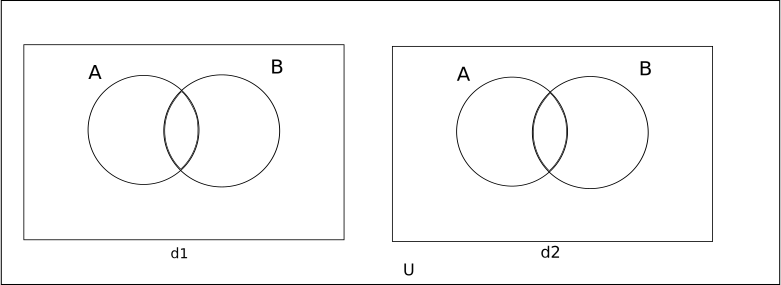
\includegraphics[scale=0.7]{images/d7.png}
\caption{Two diagrams in the universe}
\label{d7}
\end{figure}

Clearly the intersection of $d_{1}$ and $\neg d_{1}$ which means the common elements between $d_{1}$ and all that is not it $d_{1}$ (its complement) is empty. Also the union of $d_{1}$ with all that is not in $d_{1}$ (its complement) is the universe which means $d_{1}$ and $d_{2}$ and all other elements that exist in U.\\
Note that the reverse of this law is also correct which is represented by $\longleftrightarrow$ .

\subsubsection{De Morgan's Laws}
These laws say that if a compound diagram is neglected and the connector between the diagrams is a $\vee$ operator is the same as the neglect of the first diagram connected with a $\wedge$ and the neglect of the second diagram. Also if a compound diagram is neglected and the connector between the diagrams is a $\wedge$ operator is the same as the neglect of the first diagram connected with a $\vee$ and the neglect of the second diagram.
$$ \neg(d_{1} \vee d_{2}) \longleftrightarrow \neg d_{1} \wedge \neg d_{2} $$

$$ \neg(d_{1} \wedge d_{2}) \longleftrightarrow \neg d_{1} \vee \neg d_{2} $$

De Morgan's law can also be explained using union and intersection operators. 
\subsection{Unitary Diagram Proving Algorithm}

\subsection{Compound Diagram Proving Algorithm}



\section{Design}

\section{Implementation}

\section{Testing}

\section{Conclusion}
\subsection{Lessons Learnt}
\subsection{Future Work}
\newpage
\bibliographystyle{plain}	
\bibliography{refs}		% expects file "refs.bib"
\end{document}